\subsection{トランスパイラ}
先行研究\cite{miyamoto-master}では,モデルに依存するパラメータを調節するために,
計算モデルが記述されたMODファイルからnmodlを介して生成されたCファイルを手動で変更を加えることで最適化を図っていた.\\
本研究では,自動チューニングを目的としているため,このプロセスも自動化する必要があり,そのためにこのMODからCへ変換するトランスパイラを作成した.\\
MODをパースするにあたってはDomain-Specific Languagesを作成するためのPythonライブラリである,textX ( TODO: ref)を利用し,
またMODのContext Free GrammarはMODファイルからNeuroMLを生成するためのプロジェクトであるpynmodl ( TODO: ref)のプログラムを用いた.\\

\subsubsection{nmodl}
NEURONに付属しているトランスパイラであるnmodlは,MODファイルをlexとyacc ( TODO: lex yaccの参照)を用いてパースした情報を
C言語のテンプレートに埋め込むことで対応するC言語のファイルを出力している.\\
このテンプレート化された部分の中にはNEURON本体とリンクさせるために必要な情報も多数あるため,
本研究で作成するトランスパイラもnmodlのC言語テンプレートをベースに利用した.\\
( TODO: もう少し説明をたす)

\subsubsection{textX}
MODファイルから抽象木を構築するために, Domain Specific Language(以下DSL)作成用のPythonライブラリであるtextX\cite{textX}を用いた.
DSLとは, C言語等に代表される汎用言語ではなく, 微分方程式の記述を行うMODファイルのように応用先が特定の領域に限られる言語である.\\
一般的に言語を作成しようとした時, Lexer, ParserそしてCode generationという3つの機能を実装する必要がある.
しかしながら, 言語のメタモデルを作成することでtextXは内部的にLexerとParserの役割を果たすため,
メタモデルを記述したファイル(.txという拡張子を用いる)と, メタモデルから生成された抽象木からコードを生成するプログラムを実装することでDSLに対するコンパイラを作成することができる.\\
また, MODファイルのメタモデルは前述したpynmodlというプロジェクトで作成されたものを用いた.\\
図\ref{fig:hh-mod-ast}はHodgkin-HuxleyのMODファイルの抽象木を表しており, 以下textXから得られた抽象木からC言語のプログラムを生成する方法について述べる.\\

\begin{figure}[htb]
% h:here, t:top, b:bottom, p:page
  \begin{center}
    \includegraphics[width=10.0cm, angle=-90]{./images/hh-mod.pdf}
    \caption{Hodgkin-HuxleyのMODファイルの抽象木}
    \label{fig:hh-mod-ast}
  \end{center}
\end{figure}~\\
\clearpage

\subsubsection{構成}
( TODO: 章番号)のアルゴリズムで触れた中で,トランスパイラ内で実装を行ったのはモデルに依存するパラメータであり,
NEURON本体で細胞単位での計算の並列化等の設定もできるため,主に逐次プログラムの最適化を主眼に置いた.\\

MODファイルをC言語のファイルに変換する際,変換されたC言語のファイルは,\\
\begin{enumerate}
\item nmodl内でテンプレート化されている共通部分(base)
\item グローバル変数や関数定義部分(definition)
\item それぞれの関数や変数をNEURONとリンクさせる部分(register)
\item ユーザー定義関数部分(user)
\item NEURON本体と関連する関数部分(neuron)
\item ODE(微分方程式)を計算する関数部分(ode)
\end{enumerate}
の6つに分けることができる.\\

\begin{figure}[htb]
% h:here, t:top, b:bottom, p:page
  \begin{center}
    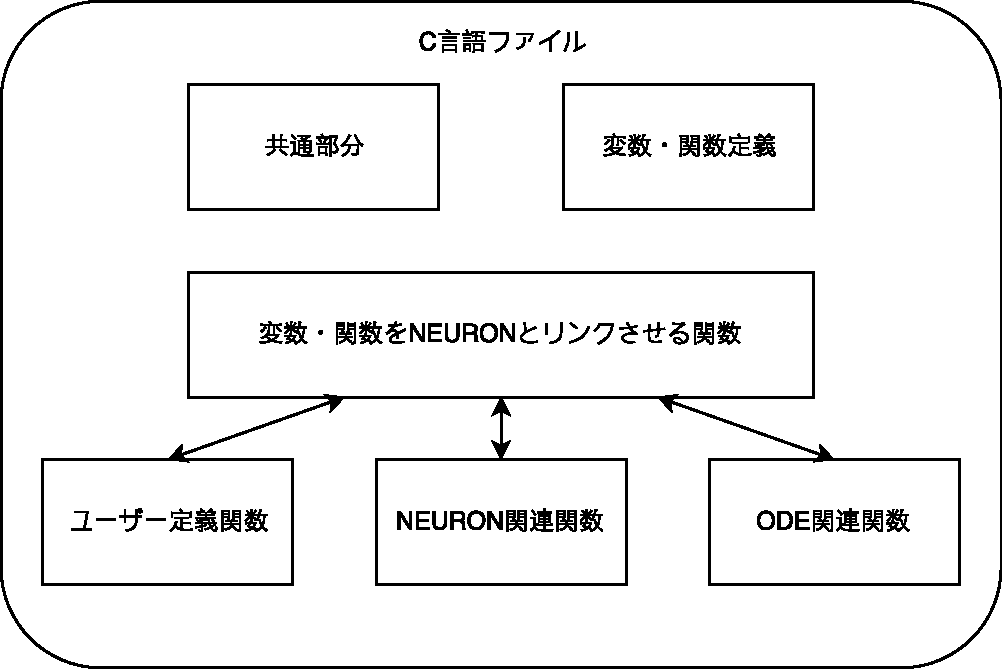
\includegraphics[width=10.0cm]{./images/transpiler-c-file.pdf}
    \caption{変換されたC言語ファイルの構成}
    \label{fig:transpiler}
  \end{center}
\end{figure}~\\

この中で計算を行うのは4, 5, 6の部分であるが, これらは2や3の部分を通して疎に繋がってはいるものの,
互いに独立性が非常に高い.\\
そのため, それぞれに対して個別に最適化を行い最終的に組み合わせてC言語のファイルを生成する方法を取ることができる.\\
本研究では図\ref{fig:transpiler}のように, まずtextXを用いてMODファイルから抽象木を生成し,
その抽象木を解析することで最適化に用いるパラメータの候補を生成したのち,
それらのパラメータと抽象木から個々に最適化を行ったものをテンプレートに埋め込むことで対応するC言語のファイルを生成した.\\

またこのようにC言語に変換する部分と抽象木自体を解析する部分を完全に分離するだけでなく,
それぞれ内部でさらに役割ごとに分割することで,最適化の方法を追加する際にも変更しやすくなる.\\
仮にこれらがすべて密に繋がっていた場合, 新しい方法を追加するためには関連する箇所をすべて正確に変更する必要があり,
規模が大きくなるにつれて難しくなっていくが, 細かく担当する範囲を分割していることで例えばODEのみに関連する変更を加えたい場合は,
ODEを担当するモジュールのみの変更でよくなる.\\
さらに, それぞれのモジュールが抽象木の情報とパラメータを直接受け取るため, モジュールごとに細かい最適化を行うことができるとともに,
シミュレータからもどの最適化をどの関数に適用するといった場合分けをしやすくなる.\\

\begin{figure}[htb]
% h:here, t:top, b:bottom, p:page
  \begin{center}
    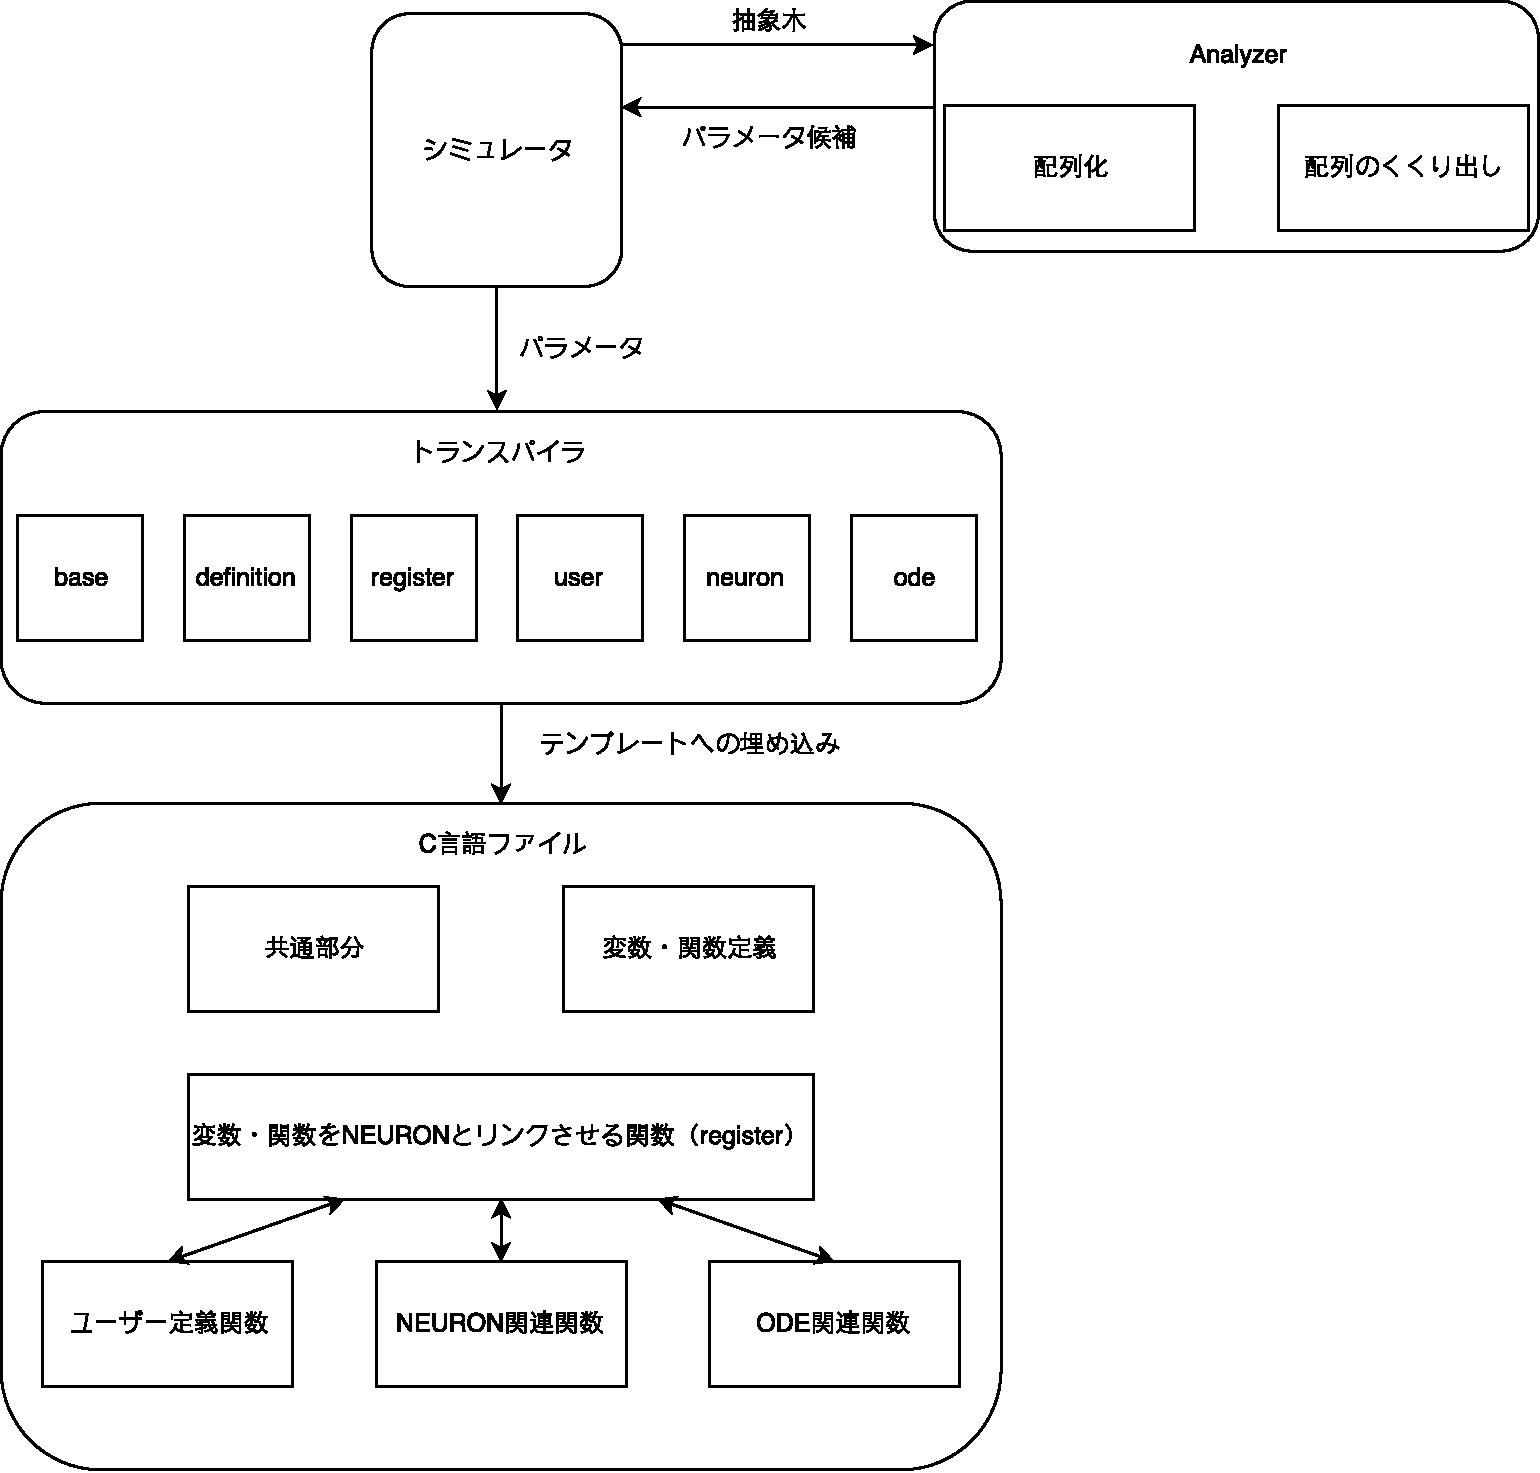
\includegraphics[width=1.1\textwidth]{./images/transpiler-image.pdf}
    \caption{トランスパイラ 構成}
    \label{fig:transpiler}
  \end{center}
\end{figure}~\\

\clearpage

\paragraph{変数の取り出し}~\\
SIMD化と配列のくくり出しを行うために, MODファイルの中で利用されている変数を取り出す必要がある.\\
これは前述のhh.modを例にすると,
{\footnotesize
\begin{lstlisting}[caption=Hodgikin-Huxleyモデルの計算式,label=hh-mod-calc,numbers=none]
? interface
NEURON {
  GLOBAL minf, hinf, ninf, mtau, htau, ntau
}

? currents
BREAKPOINT {
  SOLVE states METHOD cnexp
  gna = gnabar * m * m * m * h
	ina = gna * (v - ena)
  gk = gkbar * n * n * n * n
	ik = gk * (v - ek)
  il = gl * (v - el)
}

? states
DERIVATIVE states {
  rates(v)
  m' = (minf - m) / mtau
  h' = (hinf - h) / htau
  n' = (ninf - n) / ntau
}
\end{lstlisting}
}
の部分から取得できることがわかる.\\
pynmodlでパースした抽象木では, Breakpoint, Derivative, Globalという名前がつけられているためそれぞれの式は抽象木のrootをrootという変数で保持しているとすると,
{\footnotesize
\begin{lstlisting}[caption=計算式の取得,label=obtain-vars,numbers=none]
derivative_stmts = children_of_type('Derivative', root)[0].b.stmts
breakpoint_stmts = children_of_type('Breakpoint', root)[0].b.stmts
\end{lstlisting}
}
として取得することができる.\\
また, これらの式から変数を取得するには,
{\footnotesize
\begin{lstlisting}[caption=変数の取得,label=obtain-vars,numbers=none]
# 式を変数に分離する
parse_into_token(exp) {
    # 変数の区切りとなる文字の定義
    term_exp = re.compile("[\(\)\+\-\/\*\=\{\}\s]")
    start = 0
    pos = 0
    tokens = []
    # 末尾が変数名で終わる時のために空白を追加する
    exp += " "
    while pos < exp.size() {
        # 区切り文字であるかの確認
        m = term_exp.match(exp[pos])
        if m {
            # 変数名の取得
            token = exp[start:pos]
            # 空文字でなければ変数名のリストに追加
            if token.size() > 0 {
                tokens.append(token)
            }
            # 変数名の開始位置を更新
            start = pos + 1
        }
        pos += 1
    }
    return list(set(tokens))
}

get_symbols(path, stmts) {
    symbols = []
    for stmt in stmts {
        tokens = []
        # 式の左辺から変数名を取得
        if hasattr(stmt, 'variable') {
            if stmt.variable {
                if hasattr(stmt.variable, 'lems') {
                    exp = stmt.variable.lems
                } else {
                    exp = stmt.variable
                }
                tokens_lhs = parse_into_token(exp)
                if len(tokens_lhs) {
                    tokens.append(tokens_lhs)
                }
            }
        }
        # 式の右辺から変数名を取得
        if hasattr(stmt, 'expression') {
            if stmt.expression.lems {
                tokens_rhs = parse_into_token(stmt.expression.lems)
                if len(tokens_rhs) {
                    tokens.append(tokens_rhs)
                }
            }
        }
        # 変数名の中で重複するものがある場合は重複しているものを削除する
        if len(tokens) {
            symbols.append(list(set(tokens)))
        }
    }
    return symbols
}
\end{lstlisting}
}
とすることで取得でき, DerivativeとBreakpointそれぞれに含まれる式を引数とすることで変数名のリストを取得できる.\\

\paragraph{SIMD化}~\\
SIMD化をするためには, 計算式の中で用いられてる変数を配列化する必要がある.\\
ここで必要となるのは,
\begin{enumerate}
\item 配列を定義する
\item 計算式の変数名を配列名に変更する
\end{enumerate}
の2点である.\\
これは変数を取得したのちに, SIMD化を行う変数を選択し式の中で該当する変数を配列化すれば良い.\\
本研究において配列名は, \_変数名\_tableとして定義することとする.\\
{\footnotesize
\begin{lstlisting}[caption=計算式内の変数の配列化,label=obtain-vars,numbers=none]

get_simdize_table(root, token_list) {
    code = ""
    # SIMD 化する変数のリストそれぞれに対応する配列を定義する
    for token in token_list {
        code += "static double _{0}_table[BUFFER_SIZE * MAX_NTHREADS];\n"\
                .format(token)
    }
    return code
}

simdize_exp(exp, token_list) {
    # SIMD 化を行った後の式を保持する変数
    simdized_exp = ""
    term_exp = re.compile("[\(\)\+\-\/\*\=\{\}\s]")
    start = 0
    pos = 0
    tokens = []
    exp += " "
    while pos < exp.size() {
        m = term_exp.match(exp[pos])
        # 区切り文字であるかの確認
        if m {
            # 変数名の取得
            token = exp[start:pos]
            if token {
                # もし変数名が SIMD 化する対象であるならば配列名に置き換える
                if token in token_list {
                    simdized_exp += "_{0}_table[_iml]"\
                                     .format(token)
                } else {
                    simdized_exp += token
                }
            }
            # 区切り文字は元の式を構成するために必要なので変数名の後に追加する
            simdized_exp += exp[pos]
            start = pos + 1
        }
        pos += 1
    }
    # 区切り文字の空白を最後尾に追加しているので, 空白を抜かして返す
    return simdized_exp[:simdized_exp.size() - 1]
\end{lstlisting}
}

\paragraph{配列構造のくくり出し}~\\
アルゴリズムの章( TODO : 章番号)において,Union-Find木を用いてMODファイル内の式を分類することで,
配列としてくくり出せる変数をグループ化する手法について述べた.\\
グループ化された変数をもとに配列をくくり出す際, 配列に対するアクセス方法が変わってしまうため対応する箇所をすべて変更しなければならないという
問題が生じた. そこで, 配列へのアクセスをマクロを通して行うことで同一の方法でくくり出した配列にもアクセスできるようにした.\\
{\footnotesize
\begin{lstlisting}[caption=計算式内の変数の配列化,label=obtain-vars,numbers=none]

get_optimize_table(token_list, merge_table_list) {
    """
    " token_list: 配列化する変数名のリスト [変数1, 変数2,...]
    " merge_table_list: くくり出しを行う変数名のリスト [[変数1, 変数2, ...], [変数3, 変数4, ...], ...]
    """
    code = ""
    if merge_table_list {
        for i = 0 to merge_table_list.size() {
            # くくり出しを行う変数のグループそれぞれの大きさ分の配列を確保する
            code += "static double opt_table{0}"\
                    "[BUFFER_SIZE * MAX_NTHREADS][{1}];\n"\
                    .format(i, merge_table_list[i].size())

            # それぞれの変数に対して一意にアクセスできるようにマクロを定義する
            for j = 0 to merge_table_list[i].size() {
                code += "#define TABLE_{0}(x) "\
                        "opt_table{1}[(x)][{2}]\n"\
                        .format(merge_table_list[i][j].upper(), i, j)

                # くくり出しを行った配列はすでに定義済みであるため, 配列化するリストから除外する
                if merge_table_list[i][j] in token_list {
                    token_list.remove(merge_table_list[i][j])
                }
            }
        }
    }
    # くくり出しが行われなかった変数に対しても同様に配列とその配列にアクセスするためのマクロを定義する
    for token in token_list {
        code += "static double _{0}_table[BUFFER_SIZE * MAX_NTHREADS];\n"\
                .format(token)
        code += "#define TABLE_{0}(x) _{1}_table[(x)]\n"\
                .format(token.upper(), token)
    }
            code += "static double _{0}_table[BUFFER_SIZE * MAX_NTHREADS];\n"\
                    .format(param)
    return code
}

optimize_exp(exp, token_list, merge_table_list) {
    optimized_exp = ""
    term_exp = re.compile("[\(\)\+\-\/\*\=\{\}\s]")
    start = 0
    pos = 0
    tokens = []
    exp += " "
    while pos < exp.size() {
        m = term_exp.match(exp[pos])
        # 区切り文字であるかの確認
        if m {
            # 変数名の取得
            token = exp[start:pos]
            if token {
                # 変数が SIMD 化またはくくり出しを行う対象であるならばマクロに置き換える
                if token in merge_table_list or token in token_list {
                    optimized_exp += "TABLE_{0}(_iml)"\
                                     .format(token.upper())
                } else {
                    optimized_exp += token
                }
            }
            # 区切り文字は元の式を構成するために必要なので変数名の後に追加する
            optimized_exp += exp[pos]
            start = pos + 1
        }
        pos += 1
    }
    # 区切り文字の空白を最後尾に追加しているので, 空白を抜かして返す
    return optimized_exp[:optimized_exp.size() - 1]
}
\end{lstlisting}
}
